%%%%%%%%%%%%%%%%%%%%%%% file typeinst.tex %%%%%%%%%%%%%%%%%%%%%%%%%
%
% This is the LaTeX source for the instructions to authors using
% the LaTeX document class 'llncs.cls' for contributions to
% the Lecture Notes in Computer Sciences series.
% http://www.springer.com/lncs       Springer Heidelberg 2006/05/04
%
% It may be used as a template for your own input - copy it
% to a new file with a new name and use it as the basis
% for your article.
%
% NB: the document class 'llncs' has its own and detailed documentation, see
% ftp://ftp.springer.de/data/pubftp/pub/tex/latex/llncs/latex2e/llncsdoc.pdf
%
%%%%%%%%%%%%%%%%%%%%%%%%%%%%%%%%%%%%%%%%%%%%%%%%%%%%%%%%%%%%%%%%%%%


\documentclass[runningheads,a4paper]{llncs}

\usepackage{amssymb}
\setcounter{tocdepth}{3}
\usepackage{graphicx}
\usepackage{epstopdf}
\usepackage{subfig}
\usepackage{array}
\usepackage{xcolor}

\graphicspath{{images/}}

\usepackage{url}
\urldef{\mailsa}\path|ary506@york.ac.uk|
\newcommand{\keywords}[1]{\par\addvspace\baselineskip
\noindent\keywordname\enspace\ignorespaces#1}

\begin{document}

\mainmatter  % start of an individual contribution

% first the title is needed
\title{Gamification of Software Modelling Learning}

% a short form should be given in case it is too long for the running head
\titlerunning{Gamification of Software Modelling Learning}

% the name(s) of the author(s) follow(s) next
%
% NB: Chinese authors should write their first names(s) in front of
% their surnames. This ensures that the names appear correctly in
% the running heads and the author index.
%
\author{Alfa Yohannis \and Dimitris Kolovos \and Fiona Polack} %FACP: I've added our names (it's conventional to include supervisors in the author list).  I'm not sure how they want author lists formatting, so you might need to edit.
%
\authorrunning{Gamification of Software Modelling Learning}
% (feature abused for this document to repeat the title also on left hand pages)

% the affiliations are given next; don't give your e-mail address
% unless you accept that it will be published
\institute{Department of Computer Science, University of York, York, United Kingdom\\
\mailsa\\}

%
% NB: a more complex sample for affiliations and the mapping to the
% corresponding authors can be found in the file "llncs.dem"
% (search for the string "\mainmatter" where a contribution starts).
% "llncs.dem" accompanies the document class "llncs.cls".
%

\toctitle{Lecture Notes in Computer Science}
\tocauthor{Gamification of Software Modelling Learning}
\maketitle

\begin{abstract}
Software modelling has a fundamental role in software engineering. However, it is  perceived as difficult for learners to develop the necessary abstraction skills to master the subject. Gamification is  flourishing as a  popular strategy to engage learners. Our research exploits gameful design as an innovative approach, used to create games that reinforce learners' mastery of software modelling by developing their abstraction skills. Our approach to gameful design brings together gamification development concepts such as design lenses and intrinsic skill atoms, and pedagogical design principles from  learning theories and models.  The research follows the Design Science Research Methodology and exploits Model-Driven Engineering best practice.  To date, the research has developed a prototype for learning software modelling through gamification. Evaluation of the artefact will use longitudinal controlled experiments.
\keywords{software modelling, gamification, learning, abstraction}
\end{abstract}

\section{Introduction}
Software modelling is commonly perceived as a difficult subject since it requires a mastery of abstraction \cite{Borstler2012}. However, this subject is crucial to software engineering education and practice. Failure to master modelling affects the student’s abstraction capability in analysing and designing real-world software. Weak software modelling may cause software engineering students difficulties in completing their degrees, as most of the software engineering related subjects have a sense of intrinsic abstraction  \cite{Kramer2007}. Students' perception of software modelling  affects their attitude towards software engineering  and their career paths in the future.

The problem of learning appropriate abstraction skills is similar in software modelling and in mathematics, where most of the concepts can only be accessed through symbolical representation \cite{Duval2006}. Abstraction also requires  students to perform information hiding, generalisation, and approximation or reformulation, leaving out the irrelevant aspects but keeping the relevant ones, and separating from the concrete reality \cite{Saitta2013}. To overcome these challenges, we need to put  effort into designing delivering software modelling training, developing a motivating presentation that can engage students and facilitate deep learning.

Recently, the use of games or game elements for serious purposes other than leisure has drawn much attention. Gamification \cite{deterding2011game} and Serious Games \cite{Michael2005} have been viewed as solutions to motivational problems that emerge when users are required to engage in activities that they perceive as boring, irrelevant or difficult, e.g. learning sorting algorithms \cite{Yohannis2015} or C-programming \cite{Ibanez2014}.

The purpose of this research is to investigate and develop a gamification design framework that systematically and semi-automatically drives gamification design to produce well designed software modelling games. More precisely, this research aims to answer the following research questions:
\begin{enumerate}
\item Which processes, aspects, principles, or components of software modelling and its teaching and learning practices should be included?
\item What types of game elements and  roles  can deliver software modelling learning best? 
\item What kind of  orchestrating framework is needed to design the interaction between software modelling and game elements?
\item To what extent does gamification of software modelling improve engagement, motivation and  learners’ performance?
\end{enumerate}

\section{Related Work}
Approaches that attempt to bring software modelling into a  concrete presentation that can be easily understood by learners, range from didactic learning \cite{moisan2009teaching}, modelling tools utilization \cite{Akayama2013}, alternative communication channels and the use of modelling language \cite{Brandsteidl2011}, immersive visual modelling, through virtual environment \cite{neubauer2003immersive}, software design studio \cite{Whittle2014}, project-based approach \cite{Szmurlo2007}, to code generation investigation \cite{schmidt2014teaching}. However, most  approaches have weaknesses in motivating learners to engage continuously and actively to learn software modelling, which is a key aspect of learning \cite{Naps2005}. % To address lack of engagement, we investigate game-based learning, to learn or teach software modelling. This method provides students with a new way of learning software modelling, which is not only interactive but also engaging enough to keep them learning continuously. 
%FACP: I think this does not belong in related work and has been said clearly in the previous section.

The use of game elements for a purpose other than leisure is called gamification \cite{deterding2011game}. Gamification design is still new \cite{Deterding2013}, and, to date, there is no  design framework that specifically relates to software modelling gamification; a framework that integrates game specific domain into software modelling. % Our research aims to develop a gamification design framework of software modelling learning.%FACP: Again, I think this comment does not belong in related work.
Gamification for software engineering focuses on aspects such as software implementation and project management \cite{Pedreira2015}.  For modelling, there is work on activity diagrams, \cite{Richardsen2014}, coupling and cohesion \cite{Stikkolorum2014}, and enterprise architectures \cite{Groenewegen2010,Ionita2015}, but no general work on gamification for modelling or for learning of abstraction skills. Most papers cover the pedagogical aspect superficially, and validation is restricted to small groups of users.

\section{Research Methods}
Our research will designed artefacts, so we follow  Design Science Research Methodology (DSRM) \cite{peffers2007design}. DSRM  provides a comprehensive conceptual framework addressing the full research process. It  provides six activity guidelines for understanding, developing, executing, and evaluating design artefacts: (1) problem identification and motivation activity, (2) definition of objectives for a solution activity, (3) setting of targets for a solution activity, (4) design and development activity, (5) demonstration and evaluation activities, and (6) communication. 

Within the high-level DSRM framework, we  employ other research methods appropriate to each activity. For example, we use interviews, literature review and discussion with experts for the problem identification and motivation activity, and Deterding's lens of intrinsic skill atoms \cite{deterding2015lens} to produce a gameful design in the design and development activity.

\section{Gamification Design}
To deliver a gameful experience while playing with the artefact, game elements have to be embedded in the artefact design. Thus, design lenses and skill atoms \cite{deterding2015lens} are used to determine the required game elements and game mechanics. 

\subsection{Design Lenses}
Deterding et al.  \cite{deterding2015lens} define various design lenses, to focus analysis of the game requirements.  Here, we outline those relevant to our gamification design, and explain how they are applied to  modelling tasks.

\textbf{Challenge Lens}. The levels of the game are designed to have gradually increasing difficulty and varied challenges; the aim is to expose learners to different domains, models and diagrams. The onboarding game element is planned to be implemented into the artefact to help learners familiar with the control system and  flow of the game. The game design will also use templates to help learners build models without starting from scratch. The foundation model is  given: learners  need extend the model to meet the level's objectives.

\textbf{Goal and Motivation Lens}. The design includes interim goals and intrinsic rewards to motivate learners. For software modelling, each form of modelling (e.g. object modelling, collaboration modelling) has several stories. A story represents a specific case study to introduce learners to  problems in specific domains. Every story consists of several levels, and every level has one or more objectives that a student needs to accomplish to complete the level. The level also might be a continuation of a previous level, giving the learner a sense of step-by-step progress to complete the domain problems. Each story or level introduces new concepts as well as combining old and new concepts. Thus, as the learners progress, their competence in modelling is  developed, giving an intrinsic reward. 

\textbf{Action and Object Lens}. To help the learners to focus on the key concepts, extraneous activities that are not relevant to the core concepts should be removed.  Game elements are selected to facilitate learning the core activities: bite-sized actions (e.g. drag and drop), limited choices (e.g. only some draggable items), and microflow (e.g. put the  element in its right place). Some under-determination is used to provoke learners' creativity, since usually there is more than one possible solution model. Attractive design is  important in attracting learners' attention to interaction with the artefact.

\textbf{Feedback}. The system should give immediate, glanceable, actionable feedback to keep learners on track and monitor the state of the game. Interesting and varied feedback should be designed, to appeal to the learners' motives. 

\subsection{Intrinsic Skill Atoms}
The design of the cycle of the game mechanics is derived from intrinsic skill atoms \cite{deterding2015lens}, which requires definition of six components: motivation, goals, actions and objects, challenges, rules, and feedback. The main \emph{motivation} for engaging with our game artefact is to master software modelling, which means being able to construct models and solve model-related problems. For instance, students should be able to build an object model for a sign-in screen. The \emph{goal} of the modelling activities is to meet the given objectives whilst obeying the \emph{rules}. For example, learners are asked to construct an object diagram showing a button that, when pressed, clears a textbox; there are button  and textbox objects; the diagram is completed by linking the buttons  to represent their relationship. 

Learners are required to take  \emph{actions} to manipulate  \emph{objects} in order to achieve the modelling \emph{goals}. The artefact requires learners to  drag and  drop diagram elements to construct a model.  Draggable items include the names or values of slots, actions, and classes of objects which must be associated to the appropriate diagram elements. There are    \emph{challenges} in the form of problem-solving  to make the modelling activity more exciting. For example, an animation  shows how a login page works, and learners are asked to model it. 

All created models must adhere to the \emph{rules} that are inherent to the type of  model.  However, the game may relax  rules to avoid demotivation. For instance, a link in an object diagram should connect two objects, but this rule can be waived if linkage is not a goal or the current task. Finally, \emph{feedback} helps learners to keep track of every action  made,  informs them of their progress, and  motivates them in their ups and downs.

\section{Visual Modelling Editor}
To support developers in the design and customisation of gamification for software modelling learning at a high level of abstraction, and to automatically build a game generator, we are developing a visual modelling editor using Eugenia, a GMF-based graphical model editor \cite{kolovos2015eugenia}. Currently, developers can use the editor to design the gamification of software modelling learning by defining its flows, levels, challenges, and objectives. In  future, we plan to add  features such as user-customised types of modelling and diagram. 

\section{Evaluation}
The evaluation of the game artefact will use controlled experiments. Software modelling students will form a control group and an experimental group. The control group will learn using traditional methods; the experimental group will learn with support from the artefact. After some time learning, both groups will be given problems to solve. Their performance will be measured by their ability to solve the problems. To anticipate the order effect, students will swap then groups, and their ability will be tested again using similar problems.  To evaluate the generality of the effect of using the artefact, a longitudinal experiment is planned, and the experiments will be run in different countries and universities. The evaluation of the gamification design framework will be similar, but will target software developers and software modelling gamification construction.

The controlled experiments cannot provide understanding of why learning supported by the artefact is better or worse than the traditional approach. Therefore we plan to conduct surveys or interviews to investigate the underlying processes.   We can also investigating the artefact's event logs using data mining or machine learning techniques.   Structural equation modelling \cite{hair2016primer} would allow us to measure the effects of the identified underlying factors.  

\section{Conclusion}
This paper summarises our research problem and motivation, proposed solution and objectives, research methods, and progress on the development of the artefact.  The evaluation plan has been explained. We have omitted some  aspects of the research due to the limitation of space, such as the architecture of the artefact and the validation methods applied to evaluate models created by learners.   Whilst the current research is focusing  on software modelling, we plan to extend this to learning metamodelling and model transformation. 

\subsubsection*{Acknowledgements.} Thanks to York Masters students who  participated in our preliminary surveys. This research is supported by \emph{Lembaga Pengelola Dana Pendidikan Indonesia} (Indonesia Endowment Fund for Education). 

\bibliography{references} 
\bibliographystyle{ieeetr}

\clearpage
\section{Appendix A: Tables and Images}

\begin{table}[htb]
\caption{Design lenses (game elements) applied in the gamification design.}\label{Table001}
\begin{center}
    \begin{tabular}{ | p{3.2cm} | p {8.7cm} | }
    \hline
	\textbf{Lenses} & \textbf{Elements}\\    
    \hline
    Challenges & Onboarding, scaffolded challenge, varied challenge \\    
    \hline
    Goals and Motivation & interim goals, intrinsic rewards\\
    \hline
	Actions and Object & bite sized actions, limited choices, microflow, under-determination, sensual \\
    \hline
    Feedbacks & Immediate, juicy, actionable, appeal to motives, glanceable, varied, graspable progress\\
    \hline
    \end{tabular}
\end{center}
\end{table}

\begin{table}[htb]
\caption{Skill Atoms applied in the gamification design.}\label{Table002}
\begin{center}
    \begin{tabular}{ | p{3.2cm} | p {8.7cm} | }
    \hline
	\textbf{Atoms} & \textbf{Description}\\    
    \hline
    Motivation & Master the modelling (solve problem, able to construct model) \\    
    \hline
    Goals & Create models that satisfy requirements \\
    \hline
	Actions and Objects & Construct model using diagrams, elements of a diagram, keywords, hints \\
    \hline
    Challenges & Satisfy requirements, meet objectives\\
    \hline
	Rules & Inherent rules in every model diagram, constraints, objectives\\
	\hline
	Feedbacks & completed objectives, model metrics, and motivating words\\
	\hline
    \end{tabular}
\end{center}
\end{table}

\begin{figure}[htb]
\centering
\subfloat[Level Selection]
	{\frame{\includegraphics[height=3.5cm]{levels}}\label{Figure001}}
\hspace*{\fill}
\subfloat[Positive Reinforcement]
	{\frame{\includegraphics[height=3.5cm]{positive}}\label{Figure002}}
	\caption{Game and learning elements embedded into the artifact.}
\end{figure}

\begin{figure}[htb]
\centering
\frame{\includegraphics[width=\textwidth]{game-annotated}}
\caption{The game's display.}
\end{figure}

\begin{figure}[htb]
\centering
\frame{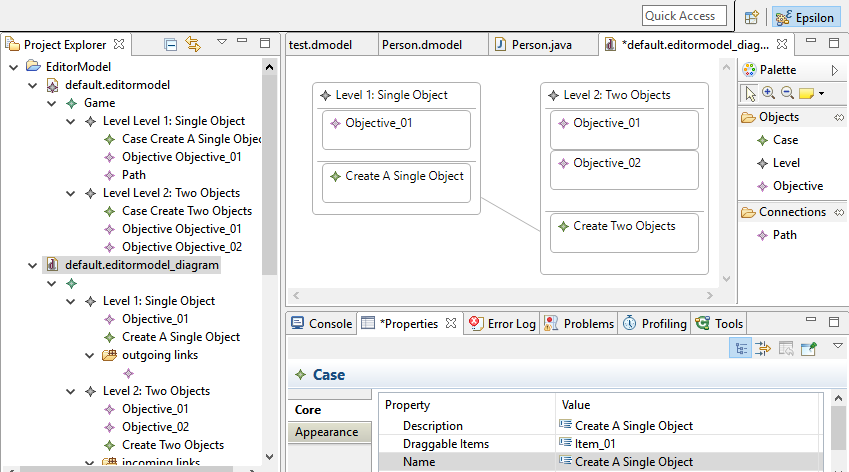
\includegraphics[width=\textwidth]{editor}}
\caption{Game editor to automatically generate the game.}
\end{figure}

\end{document}


